%%-*-latex-*-

\documentclass[11pt,a4paper]{article}

/home/rinderkn/LaTeX/TeX/trace.tex

\title{Final examination\\ of Introduction to Networking}

\author{Christian Rinderknecht}
\date{17 June 2005}

\usepackage[english]{babel}
\usepackage{vaucanson-g}
\usepackage{amsmath,amssymb}
\usepackage{clrscode}
\usepackage{graphicx}

\newcommand\type[1]{\textsf{#1}}

\begin{document}

\maketitle

\section{Binary tree specification}

Let us recall an algebraic specification of binary trees over
nodes. Let us call it \(\proc{Bin-Tree}(\type{node})\). Here is the
signature:
\begin{itemize}

  \item \textbf{Defined types}

  \begin{itemize}

    \item The type of the binary trees is noted \type{t}.

    \item The type of the nodes is noted \type{node}.
  
  \end{itemize}

  \item \textbf{Constructors}
  \begin{itemize}

    \item \proc{Empty} : \type{t}\\
    The term \proc{Empty} represents the empty tree, i.e. the tree
    that contains no node.

    \item \(\proc{Make} : \type{node} \times \type{t} \times
    \type{t} \rightarrow \type{t}\)\\ The term \(\proc{Make}
    (r, t_1, t_2)\) denotes the tree whose root is \(r\), left
    subtree is \(t_1\) and right subtree is \(t_2\). Graphically:
    \begin{center}
      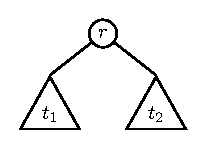
\includegraphics{non-empty_tree}
    \end{center}

  \end{itemize}

  \item \textbf{Functions}
  \begin{enumerate}

     \item \(\proc{Mem}: \type{t} \times \type{node} \rightarrow
     \type{bool}\)\\
     The term \(\proc{Mem} (t, e)\) is \proc{True} if node \(e\)
     occurs in tree \(t\), otherwise it is equal to
     \proc{False}. (We assume we have equality on nodes.)

     \item \(\proc{Min-Depth}: \type{t} \times \type{node} 
     \rightarrow \type{int}\)\\ 
     The term \(\proc{Min-Depth} (t, e)\) denotes the minimum depth at
     which node \(e\) occurs in tree \(t\). (The root is at depth 0.)
     If \(e\) is not in \(t\), the value is unspecified. In case the
     node \(e\) appears several times in \(t\), the value is the
     smallest depth of occurrence. (We assume we can compare nodes for
     equality and that we have the function \(\proc{Min}: \type{int}
     \times \type{int} \rightarrow \type{int}\) which returns the
     smallest integer argument.) For example, if \(t\) is
     \begin{center}
       \includegraphics{int_tree_example}
     \end{center}
     then \(\left\{ 
     \begin{aligned}
       \proc{Min-Depth} (t, 7) & \quad \text{is unspecified
         (i.e. undefined)}\\
       \proc{Min-Depth} (t, 1) &= 0\\
       \proc{Min-Depth} (t, 3) &= 2\\
       \proc{Min-Depth} (t, 5) &= \proc{Min} (1, 2) = 1
     \end{aligned}
     \right.\)

     \item \(\proc{Inv}: \type{t} \rightarrow \type{t}\)\\ The term
     \(\proc{Inv} (t)\) denotes the tree \(t\) in a mirror, i.e. the
     left subtrees of \(t\) are the right subtrees of \(\proc{Inv}
     (t)\) and the right subtrees become the left
     subtrees. Therefore \(\proc{Inv} (\proc{Inv} (t)) = t\). For
     example, the following trees are mirrors of each other:
     \begin{center}
       \includegraphics[bb=71 656 233 721]{mirrors}
     \end{center}

     \item \(\proc{Sum}: \proc{Bin-Tree}(\type{int}).\type{t}
     \rightarrow \type{int}\)\\
     The term \(\proc{sum} (t)\) denotes the sum of all (integer) nodes
     in tree \(t\). If \(t\) is empty, the sum is unspecified. For
     example, if \(t\) is
     \begin{center}
       \includegraphics[bb=71 656 141 721]{int_tree_example}
     \end{center}
     then \(\proc{Sum} (t) = 1 + 5 + 3 + 4 + 6 + 5 = 24\).

  \end{enumerate}

\end{itemize}


\paragraph{Question.} Design a protocol to be used between an automatic teller
machine (ATM) and a bank's centralised computer. Your protocol should
allow a user's card and password to be verified, the account balance
(which is maintained at the bank) to be queried, and an account
withdrawal to be made (money is given to the
customer). \textbf{1.~Specify your protocol} by listing the messages
exchanged and the action taken by the ATM or the bank's centralised
computer on transmission or receipt of each message:
\begin{center}
\begin{tabular}{@{}p{170pt}p{170pt}@{}}
\toprule
\multicolumn{2}{c}{From ATM to Bank}\\
\cmidrule(r{0pt}){1-2}
Message name & Meaning/Action\\
and arguments &\\
\midrule
 & \\
 & \\
 & \\
 & \\
 & \\
 & \\
 & \\
 & \\
\bottomrule
\end{tabular}

\begin{tabular}{@{}p{170pt}p{170pt}@{}}
\toprule
\multicolumn{2}{c}{From Bank to ATM}\\
\cmidrule(r{0pt}){1-2}
Message name & Meaning/Action\\
and arguments &\\
\midrule
 & \\
 & \\
 & \\
 & \\
 & \\
 & \\
 & \\
 & \\
\bottomrule
\end{tabular}
\end{center}
\noindent\textbf{2.~Sketch the operation of your protocol}, using a
diagram, for the cases of a simple withdrawal \textbf{(a)} with no
errors, \textbf{(b)} with one error.

Give the Morris-Pratt algorithm, assuming you know the supply function.


\end{document}
